%
% $RCSfile: inheritance.tex,v $
%
% Copyright (C) 2002-2008. Christian Heller.
%
% Permission is granted to copy, distribute and/or modify this document
% under the terms of the GNU Free Documentation License, Version 1.1 or
% any later version published by the Free Software Foundation; with no
% Invariant Sections, with no Front-Cover Texts and with no Back-Cover
% Texts. A copy of the license is included in the section entitled
% "GNU Free Documentation License".
%
% http://www.cybop.net
% - Cybernetics Oriented Programming -
%
% http://www.resmedicinae.org
% - Information in Medicine -
%
% Version: $Revision: 1.1 $ $Date: 2008-08-19 20:41:07 $ $Author: christian $
% Authors: Christian Heller <christian.heller@tuxtax.de>
%

\subsubsection{Inheritance}
\label{inheritance_heading}
\index{Inheritance}
\index{Superior Class}
\index{Parent Class}
\index{C++}
\index{Multiple Inheritance}
\index{Java}
\index{Single Inheritance}
\index{Interface}
\index{Application Programming Interface}
\index{API}

\emph{Inheritance} allows for code minimisation by letting classes inherit
attributes and methods from their \emph{superior} (sometimes called \emph{parent})
class (figure \ref{inheritance_figure}). Redundant code can such be avoided and
existing code can be reused. An inheriting class in \emph{Java} source code
looks like this:

\begin{scriptsize}
    \begin{verbatim}
    public class example extends super_class {
    }
    \end{verbatim}
\end{scriptsize}

\begin{figure}[ht]
    \begin{center}
        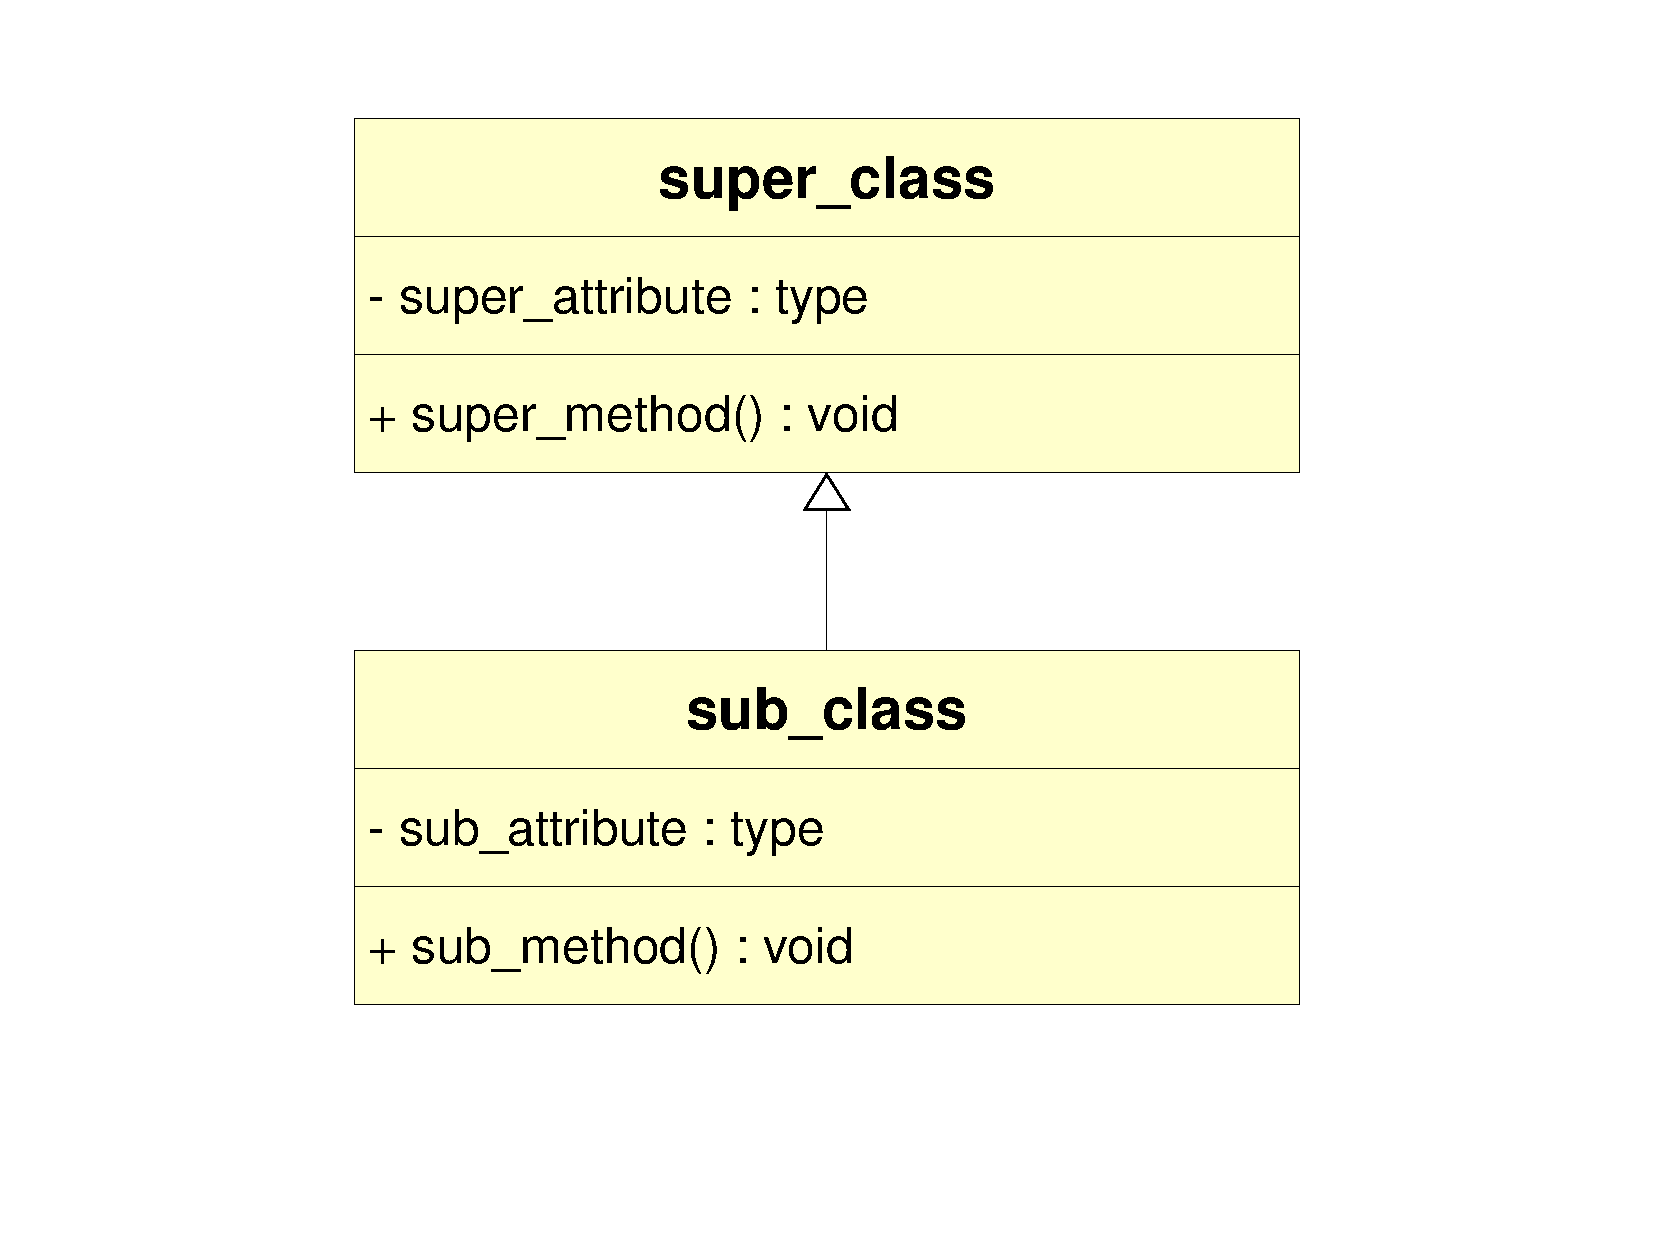
\includegraphics[scale=0.3,angle=-90]{graphic/inheritance.pdf}
        \caption{Inheritance as UML Diagram}
        \label{inheritance_figure}
    \end{center}
\end{figure}

Some object oriented programming languages (such as \emph{C++}) permit
\emph{Multiple Inheritance}. Classes written in those languages can have more
than one superior class. Other languages (such as \emph{Java}) that have
\emph{Single Inheritance} only, sometimes offer to \emph{inherit}
(\emph{realise}/ \emph{implement}) multiple interfaces. An interface forces its
subclasses to implement all methods it declares (more on this in section
\ref{interface_and_implementation_heading}) and can such provide a common
\emph{Application Programming Interface} (API) which makes classes
interchangeable and hence encourages reuse.
